\section{Trigonometrie}
Winkel in griechischen Buchstaben ($\alpha$, $\beta$ \dots) werden in $^\circ$ Grad, Winkel mit lateinischen Buchstaben ($x$, $y$, \dots) in Radian ausgedrückt.
Für Radian (= Bogenmass) gilt: der Winkel $x$ ist die Länge des Bogens $b$ im Verhältnis zum Radius $r$. Die Beziehung zwischen Grad und Radian ist:
\begin{equation*}
	\frac{\alpha}{360^{\circ}} = \frac{x}{2\pi}
\end{equation*}

In einem rechtwinkligem Dreieck mit der Hypotenuse $c$, der Gegenkathete $a$ und der Ankathete $b$ gilt:
\begin{tabular}{@{}p{\linewidth/3}%
				@{}p{\linewidth/3}%
				@{}p{\linewidth/3}}
	$\sin{\alpha} = \frac{a}{c}$ & $\cos{\alpha} = \frac{b}{c}$ & $\tan{\alpha} = \frac{a}{b} = \frac{\sin{\alpha}}{\cos{\alpha}}$\\
	%$\csc{\alpha} = \frac{c}{a}$ & $\sec{\alpha} = \frac{c}{b}$ & $\cot{\alpha} = \frac{b}{a} = \frac{1}{\tan{\alpha}}$\\
\end{tabular}
Die weiteren trigonometrischen Funktionen ($\csc\alpha = \frac{1}{\sin\alpha}$, $\sec\alpha = \frac{1}{\cos\alpha}$ und $\cot\alpha = \frac{1}{\tan\alpha}$) werden hier
nicht weiter betrachtet.

\subsection{Einheitskreis}
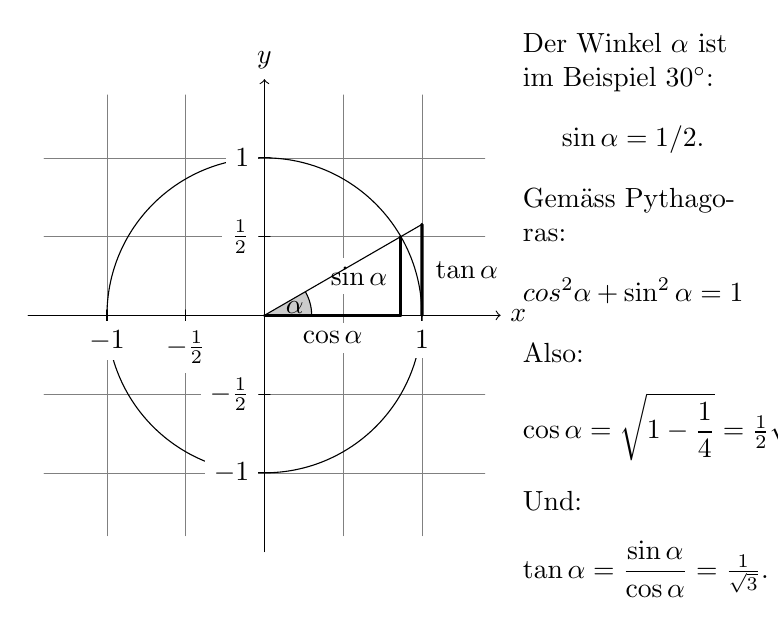
\begin{tikzpicture}[scale=2,cap=round]
  % Local definitions
  \def\costhirty{0.8660256}

  % Colors
  \colorlet{lightgrey}{white!80!black}
  %\colorlet{anglecolor}{green!50!black}
  %\colorlet{sincolor}{red}
  %\colorlet{tancolor}{orange!80!black}
  %\colorlet{coscolor}{blue}

  % Styles
  \tikzstyle{axes}=[]
  \tikzstyle{important line}=[very thick]
  \tikzstyle{information text}=[rounded corners,inner sep=0.5ex] %,fill=black!10

  % The graphic
  \draw[style=help lines,step=0.5cm] (-1.4,-1.4) grid (1.4,1.4);

  \draw (0,0) circle (1cm);

  \begin{scope}[style=axes]
    \draw[->] (-1.5,0) -- (1.5,0) node[right] {$x$};
    \draw[->] (0,-1.5) -- (0,1.5) node[above] {$y$};

    \foreach \x/\xtext in {-1, -.5/-\frac{1}{2}, 1}
      \draw[xshift=\x cm] (0pt,1pt) -- (0pt,-1pt) node[below,fill=white]
            {$\xtext$};

    \foreach \y/\ytext in {-1, -.5/-\frac{1}{2}, .5/\frac{1}{2}, 1}
      \draw[yshift=\y cm] (1pt,0pt) -- (-1pt,0pt) node[left,fill=white]
            {$\ytext$};
  \end{scope}

  \filldraw[fill=lightgrey] (0,0) -- (3mm,0pt) arc(0:30:3mm);
  \draw (15:2mm) node {$\alpha$};

  \draw[style=important line]
    (30:1cm) -- node[left=1pt,fill=white] {$\sin \alpha$} +(0,-.5);

  \draw[style=important line]
    (0,0) -- node[below=2pt,fill=white] {$\cos \alpha$} (\costhirty,0);

  \draw[style=important line] (1,0) --
    node [right=1pt,fill=white]
    {
      $\displaystyle \tan \alpha$
    } (intersection of 0,0--30:1cm and 1,0--1,1) coordinate (t);

  \draw (0,0) -- (t);

	\draw[xshift=1.6cm] node [right,text width=2.8cm,style=information text]
    {
    Der Winkel $\alpha$ ist im Beispiel $30^\circ$: 
      \[
      \sin \alpha = 1/2.
      \]
      Gemäss Pythagoras:
	  \[
	  	cos^2\alpha + \sin^2\alpha = 1
	  \]
	  Also:
      \[
      \cos\alpha = \sqrt{1 - \frac{1}{4}} = \textstyle \frac{1}{2} \sqrt 3. %
      \]%
      Und:
      \[
      \tan\alpha = \frac{\sin
          \alpha}{\cos \alpha} = \textstyle \frac{1}{\sqrt 3}.
      \]%
    };
\end{tikzpicture}

\subsubsection{Rechenregeln}
\begin{align*}
	\sin{x}& = \cos{x} + \frac{\pi}{2}\\
	\cos{x}& = \sin{x} - \frac{\pi}{2}\\
\sin(\alpha \pm \beta)& = \sin{\alpha} \cdot \cos{\beta} \pm \cos{\alpha} \cdot \sin{\beta} \\ 
\cos(\alpha \pm \beta)& = \cos{\alpha} \cdot \cos{\beta} \mp \sin{\alpha} \cdot \sin{\beta} \\
\tan(\alpha \pm \beta)& = \frac{\tan{\alpha} \pm \tan{\beta}}{1 \mp \tan{\alpha} \cdot \tan{\beta}}
\end{align*}

\subsubsection{Übersicht Eigenschaften}
\settowidth{\MyLenA}{$f^{-1'}(x)$~~}
\begin{tabular}{@{}p{\the\MyLenA}%
				@{}p{(\linewidth - \the\MyLenA)/4}%
				@{}p{(\linewidth - \the\MyLenA)/4}%
				@{}p{(\linewidth - \the\MyLenA)/4}}
	\textbf{$f(x)$}	& \textbf{$\sin x$} 					& \textbf{$\cos x$} 					& \textbf{$\tan x$}\\\hline
	$\mathbb{D}$ 	& $\mathbb{R}$ 							& $\mathbb{R}$ 							& $\mathbb{R} \backslash \{\frac{\pi}{2} + k\pi\}$\\
	$\mathbb{W}$	& $[-1, +1]$							& $[-1, +1]$							& $(-\infty, +\infty)$\\
	Peri			& $2\pi$								& $2\pi$								& $\pi$\\	
	Symm.			& ungerade								& gerade								& ungerade \\
	Null			& $x_k = k \cdot \pi$ 					& $x_k = \frac{\pi}{2} + k \cdot \pi$	& $x_k = k \cdot \pi$\\
	$f'(x)$			& $\cos x$								& $-\sin x$								& $\frac{1}{\cos^2 x}$\\
	$f^{-1}(x)$		& $\arcsin x$							& $\arccos x$							& $\arctan x$\\
	$f^{-1'}(x)$	& $\frac{1}{\sqrt{1-x^2}}$				& $-\frac{1}{\sqrt{1-x^2}}$				& $\frac{1}{1+x^2}$
\end{tabular}



